\documentclass{ximera}

%\usepackage{todonotes}

\newcommand{\todo}{}

\usepackage{esint} % for \oiint
\ifxake%%https://math.meta.stackexchange.com/questions/9973/how-do-you-render-a-closed-surface-double-integral
\renewcommand{\oiint}{{\large\bigcirc}\kern-1.56em\iint}
\fi


\graphicspath{
  {./}
  {ximeraTutorial/}
  {basicPhilosophy/}
  {functionsOfSeveralVariables/}
  {normalVectors/}
  {lagrangeMultipliers/}
  {vectorFields/}
  {greensTheorem/}
  {shapeOfThingsToCome/}
  {dotProducts/}
  {partialDerivativesAndTheGradientVector/}
  {../productAndQuotientRules/exercises/}
  {../normalVectors/exercisesParametricPlots/}
  {../continuityOfFunctionsOfSeveralVariables/exercises/}
  {../partialDerivativesAndTheGradientVector/exercises/}
  {../directionalDerivativeAndChainRule/exercises/}
  {../commonCoordinates/exercisesCylindricalCoordinates/}
  {../commonCoordinates/exercisesSphericalCoordinates/}
  {../greensTheorem/exercisesCurlAndLineIntegrals/}
  {../greensTheorem/exercisesDivergenceAndLineIntegrals/}
  {../shapeOfThingsToCome/exercisesDivergenceTheorem/}
  {../greensTheorem/}
  {../shapeOfThingsToCome/}
  {../separableDifferentialEquations/exercises/}
  {vectorFields/}
}

\newcommand{\mooculus}{\textsf{\textbf{MOOC}\textnormal{\textsf{ULUS}}}}

\usepackage{tkz-euclide}
\usepackage{tikz}
\usepackage{tikz-cd}
\usetikzlibrary{arrows}
\tikzset{>=stealth,commutative diagrams/.cd,
  arrow style=tikz,diagrams={>=stealth}} %% cool arrow head
\tikzset{shorten <>/.style={ shorten >=#1, shorten <=#1 } } %% allows shorter vectors

\usetikzlibrary{backgrounds} %% for boxes around graphs
\usetikzlibrary{shapes,positioning}  %% Clouds and stars
\usetikzlibrary{matrix} %% for matrix
\usepgfplotslibrary{polar} %% for polar plots
\usepgfplotslibrary{fillbetween} %% to shade area between curves in TikZ
%\usetkzobj{all}
\usepackage[makeroom]{cancel} %% for strike outs
%\usepackage{mathtools} %% for pretty underbrace % Breaks Ximera
%\usepackage{multicol}
\usepackage{pgffor} %% required for integral for loops



%% http://tex.stackexchange.com/questions/66490/drawing-a-tikz-arc-specifying-the-center
%% Draws beach ball
\tikzset{pics/carc/.style args={#1:#2:#3}{code={\draw[pic actions] (#1:#3) arc(#1:#2:#3);}}}



\usepackage{array}
\setlength{\extrarowheight}{+.1cm}
\newdimen\digitwidth
\settowidth\digitwidth{9}
\def\divrule#1#2{
\noalign{\moveright#1\digitwidth
\vbox{\hrule width#2\digitwidth}}}




% \newcommand{\RR}{\mathbb R}
% \newcommand{\R}{\mathbb R}
% \newcommand{\N}{\mathbb N}
% \newcommand{\Z}{\mathbb Z}

\newcommand{\sagemath}{\textsf{SageMath}}


%\renewcommand{\d}{\,d\!}
%\renewcommand{\d}{\mathop{}\!d}
%\newcommand{\dd}[2][]{\frac{\d #1}{\d #2}}
%\newcommand{\pp}[2][]{\frac{\partial #1}{\partial #2}}
% \renewcommand{\l}{\ell}
%\newcommand{\ddx}{\frac{d}{\d x}}

% \newcommand{\zeroOverZero}{\ensuremath{\boldsymbol{\tfrac{0}{0}}}}
%\newcommand{\inftyOverInfty}{\ensuremath{\boldsymbol{\tfrac{\infty}{\infty}}}}
%\newcommand{\zeroOverInfty}{\ensuremath{\boldsymbol{\tfrac{0}{\infty}}}}
%\newcommand{\zeroTimesInfty}{\ensuremath{\small\boldsymbol{0\cdot \infty}}}
%\newcommand{\inftyMinusInfty}{\ensuremath{\small\boldsymbol{\infty - \infty}}}
%\newcommand{\oneToInfty}{\ensuremath{\boldsymbol{1^\infty}}}
%\newcommand{\zeroToZero}{\ensuremath{\boldsymbol{0^0}}}
%\newcommand{\inftyToZero}{\ensuremath{\boldsymbol{\infty^0}}}



% \newcommand{\numOverZero}{\ensuremath{\boldsymbol{\tfrac{\#}{0}}}}
% \newcommand{\dfn}{\textbf}
% \newcommand{\unit}{\,\mathrm}
% \newcommand{\unit}{\mathop{}\!\mathrm}
% \newcommand{\eval}[1]{\bigg[ #1 \bigg]}
% \newcommand{\seq}[1]{\left( #1 \right)}
% \renewcommand{\epsilon}{\varepsilon}
% \renewcommand{\phi}{\varphi}


% \renewcommand{\iff}{\Leftrightarrow}

% \DeclareMathOperator{\arccot}{arccot}
% \DeclareMathOperator{\arcsec}{arcsec}
% \DeclareMathOperator{\arccsc}{arccsc}
% \DeclareMathOperator{\si}{Si}
% \DeclareMathOperator{\scal}{scal}
% \DeclareMathOperator{\sign}{sign}


%% \newcommand{\tightoverset}[2]{% for arrow vec
%%   \mathop{#2}\limits^{\vbox to -.5ex{\kern-0.75ex\hbox{$#1$}\vss}}}
% \newcommand{\arrowvec}[1]{{\overset{\rightharpoonup}{#1}}}
% \renewcommand{\vec}[1]{\arrowvec{\mathbf{#1}}}
% \renewcommand{\vec}[1]{{\overset{\boldsymbol{\rightharpoonup}}{\mathbf{#1}}}}

% \newcommand{\point}[1]{\left(#1\right)} %this allows \vector{ to be changed to \vector{ with a quick find and replace
% \newcommand{\pt}[1]{\mathbf{#1}} %this allows \vec{ to be changed to \vec{ with a quick find and replace
% \newcommand{\Lim}[2]{\lim_{\point{#1} \to \point{#2}}} %Bart, I changed this to point since I want to use it.  It runs through both of the exercise and exerciseE files in limits section, which is why it was in each document to start with.

% \DeclareMathOperator{\proj}{\mathbf{proj}}
% \newcommand{\veci}{{\boldsymbol{\hat{\imath}}}}
% \newcommand{\vecj}{{\boldsymbol{\hat{\jmath}}}}
% \newcommand{\veck}{{\boldsymbol{\hat{k}}}}
% \newcommand{\vecl}{\vec{\boldsymbol{\l}}}
% \newcommand{\uvec}[1]{\mathbf{\hat{#1}}}
% \newcommand{\utan}{\mathbf{\hat{t}}}
% \newcommand{\unormal}{\mathbf{\hat{n}}}
% \newcommand{\ubinormal}{\mathbf{\hat{b}}}

% \newcommand{\dotp}{\bullet}
% \newcommand{\cross}{\boldsymbol\times}
% \newcommand{\grad}{\boldsymbol\nabla}
% \newcommand{\divergence}{\grad\dotp}
% \newcommand{\curl}{\grad\cross}
%\DeclareMathOperator{\divergence}{divergence}
%\DeclareMathOperator{\curl}[1]{\grad\cross #1}
% \newcommand{\lto}{\mathop{\longrightarrow\,}\limits}

% \renewcommand{\bar}{\overline}

\colorlet{textColor}{black}
\colorlet{background}{white}
\colorlet{penColor}{blue!50!black} % Color of a curve in a plot
\colorlet{penColor2}{red!50!black}% Color of a curve in a plot
\colorlet{penColor3}{red!50!blue} % Color of a curve in a plot
\colorlet{penColor4}{green!50!black} % Color of a curve in a plot
\colorlet{penColor5}{orange!80!black} % Color of a curve in a plot
\colorlet{penColor6}{yellow!70!black} % Color of a curve in a plot
\colorlet{fill1}{penColor!20} % Color of fill in a plot
\colorlet{fill2}{penColor2!20} % Color of fill in a plot
\colorlet{fillp}{fill1} % Color of positive area
\colorlet{filln}{penColor2!20} % Color of negative area
\colorlet{fill3}{penColor3!20} % Fill
\colorlet{fill4}{penColor4!20} % Fill
\colorlet{fill5}{penColor5!20} % Fill
\colorlet{gridColor}{gray!50} % Color of grid in a plot

\newcommand{\surfaceColor}{violet}
\newcommand{\surfaceColorTwo}{redyellow}
\newcommand{\sliceColor}{greenyellow}




\pgfmathdeclarefunction{gauss}{2}{% gives gaussian
  \pgfmathparse{1/(#2*sqrt(2*pi))*exp(-((x-#1)^2)/(2*#2^2))}%
}


%%%%%%%%%%%%%
%% Vectors
%%%%%%%%%%%%%

%% Simple horiz vectors
\renewcommand{\vector}[1]{\left\langle #1\right\rangle}


%% %% Complex Horiz Vectors with angle brackets
%% \makeatletter
%% \renewcommand{\vector}[2][ , ]{\left\langle%
%%   \def\nextitem{\def\nextitem{#1}}%
%%   \@for \el:=#2\do{\nextitem\el}\right\rangle%
%% }
%% \makeatother

%% %% Vertical Vectors
%% \def\vector#1{\begin{bmatrix}\vecListA#1,,\end{bmatrix}}
%% \def\vecListA#1,{\if,#1,\else #1\cr \expandafter \vecListA \fi}

%%%%%%%%%%%%%
%% End of vectors
%%%%%%%%%%%%%

%\newcommand{\fullwidth}{}
%\newcommand{\normalwidth}{}



%% makes a snazzy t-chart for evaluating functions
%\newenvironment{tchart}{\rowcolors{2}{}{background!90!textColor}\array}{\endarray}

%%This is to help with formatting on future title pages.
\newenvironment{sectionOutcomes}{}{}



%% Flowchart stuff
%\tikzstyle{startstop} = [rectangle, rounded corners, minimum width=3cm, minimum height=1cm,text centered, draw=black]
%\tikzstyle{question} = [rectangle, minimum width=3cm, minimum height=1cm, text centered, draw=black]
%\tikzstyle{decision} = [trapezium, trapezium left angle=70, trapezium right angle=110, minimum width=3cm, minimum height=1cm, text centered, draw=black]
%\tikzstyle{question} = [rectangle, rounded corners, minimum width=3cm, minimum height=1cm,text centered, draw=black]
%\tikzstyle{process} = [rectangle, minimum width=3cm, minimum height=1cm, text centered, draw=black]
%\tikzstyle{decision} = [trapezium, trapezium left angle=70, trapezium right angle=110, minimum width=3cm, minimum height=1cm, text centered, draw=black]


\title{Discontinuity}

\begin{document}

\begin{abstract}
breaks
\end{abstract}
\maketitle







A \textbf{discontinuity} is the first kind of interruption in our expectations. \\


They say a picture is worth a thousand words. Here are a thousand words. \\


Graph of $y = f(x)$.

\begin{image}
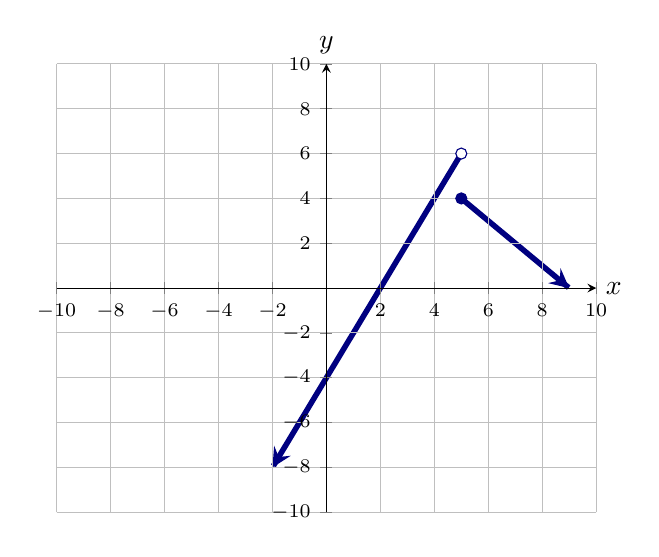
\begin{tikzpicture}
  \begin{axis}[
            domain=-10:10, ymax=10, xmax=10, ymin=-10, xmin=-10,
            axis lines =center, xlabel=$x$, ylabel=$y$, grid = major,
            ytick={-10,-8,-6,-4,-2,2,4,6,8,10},
            xtick={-10,-8,-6,-4,-2,2,4,6,8,10},
            ticklabel style={font=\scriptsize},
            every axis y label/.style={at=(current axis.above origin),anchor=south},
            every axis x label/.style={at=(current axis.right of origin),anchor=west},
            axis on top
          ]
          
          \addplot [line width=2, penColor, smooth,samples=200,domain=(-2:5),<-] {2*x-4};
          \addplot [line width=2, penColor, smooth,samples=200,domain=(5:9),->] {-x+9};

          \addplot[color=penColor,fill=penColor,only marks,mark=*] coordinates{(5,4)};
          \addplot[color=penColor,fill=white,only marks,mark=*] coordinates{(5,6)};

  \end{axis}
\end{tikzpicture}
\end{image}

The domain number $5$ is a discontinuity of $f$. \\




\subsection*{the Thousand Words}


A discontinuity in a function is first of all a domain number.  $5$ is a domain number of the function $f$ above.


The function has a value at this number. $f(5) = 4$, in the function above.




Secondly, around this domain number, the function values are not \textbf{\textcolor{purple!85!blue}{all}} close to the value at the discontinuity. There is empty space between the function value at the discontinuity and \textbf{\textcolor{purple!85!blue}{some}} of the surrounding function values - \textbf{\textcolor{red!70!black}{no matter how close you get to the discontinuity in the domain}}. \\


In the function above, no matter how close you get to $5$ in the domain, there are still domain numbers less than $5$ where $f$ has values around $6$, not $4$. You cannot get close enough to $5$ in the domain to get away from function values around $6$.



\textbf{\textcolor{red!70!darkgray}{$\blacktriangleright$}} Our job is to \link[algebraize]{https://en.wiktionary.org/wiki/algebraize} this idea. \\


Our plan is to use $\epsilon$-intervals around function values and $\delta$-intervals around domain numbers.\\




$\blacktriangleright$ \textbf{First Draft:}

Let $a$ be a discontinuity of the function $f$.  First, $a$ is in the domain of $f$. $f(a)$ exists.  $f(a)$ is a value in the range of $f$. Since $a$ is a discontinuity, there must be a distance (perhaps really small), which we'll call $\epsilon$, which defines an open interval in the codomain around $f(a)$ - namely $(f(a)-\epsilon, f(a)+\epsilon)$.  \\


And, no matter how close you get to $a$, there are domain numbers closer to $a$ where the function value is outside $(f(a)-\epsilon, f(a)+\epsilon)$. \\



No matter how small $\delta>0$ is, there is always a domain number, $b \in (a-\delta, a+\delta)$ such that $ f(b) \not\in(f(a)-\epsilon, f(a)+\epsilon)$ \\





\begin{observation}

For the function $f$ above, $5$ is a discontinuity. \\


$f(5) = 4$ and we can select the open interval $(3.5, 4.5)$ around $4$.   This would correspond to $\epsilon = 0.5$.

\[   (3.5, 4.5) = (f(5) - \epsilon, f(5) + \epsilon)    \]


No matter how close you get to $5$, no matter how small you select $\delta$, the open interval $(5 - \delta, 5 + \delta)$ contains the domain number $\frac{(5 - \delta) + 5}{2}$, where the function $f$ has a value outside $(3.5, 4.5)$.


No matter how close you get to $5$ in the domain, you cannot get \textbf{\textcolor{blue!55!black}{all}} of the function values to be close to $f(5)$.

\end{observation}



















\begin{definition} \textbf{\textcolor{green!50!black}{Discontinuity}}

The real number $a$ is a \textbf{discontinuity} of the function $f$ if

\begin{itemize}
\item $a \in Dom_f$ meaning $a$ is in the domain of $f$, which means $f(a) \in \mathbb{R}$, i.e. $f(a)$ exists.
\item There is an $\epsilon > 0$ defining an open interval around $f(a)$, namely $I = (f(a) - \epsilon, f(a) + \epsilon)$, such that for any $\delta > 0$, the open interval $(a - \delta, a + \delta)$ always contains a domain number $b$, such that $f(b) \not\in(f(a)-\epsilon, f(a)+\epsilon)$.
\end{itemize}

There is an open interval $I$ around $f(a)$, such that \textbf{\textcolor{purple!85!blue}{EVERY}} open interval around $a$ contains a domain number where the function value is outside $I$.

\end{definition}


\textbf{Discontinuity:}  When domain numbers are close, the function values are not ALL close. \\





\begin{example}


\[
\text{Let } \, f(x) = 
\begin{cases}
  2x-4 & \text{ on } (-2, 5) \\
  -x + 9  & \text{ on } [5, 9)
\end{cases}
\]


Graph of $y=f(x)$


\begin{image}
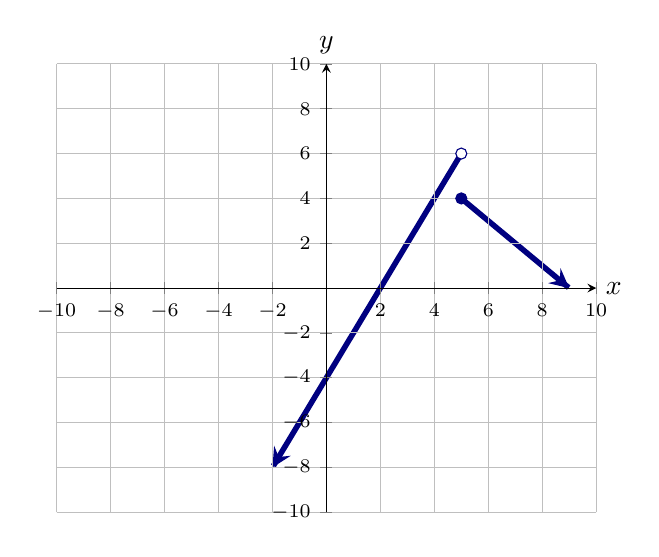
\begin{tikzpicture}
  \begin{axis}[
            domain=-10:10, ymax=10, xmax=10, ymin=-10, xmin=-10,
            axis lines =center, xlabel=$x$, ylabel=$y$, grid = major,
            ytick={-10,-8,-6,-4,-2,2,4,6,8,10},
            xtick={-10,-8,-6,-4,-2,2,4,6,8,10},
            ticklabel style={font=\scriptsize},
            every axis y label/.style={at=(current axis.above origin),anchor=south},
            every axis x label/.style={at=(current axis.right of origin),anchor=west},
            axis on top
          ]
          
          \addplot [line width=2, penColor, smooth,samples=200,domain=(-2:5),<-] {2*x-4};
          \addplot [line width=2, penColor, smooth,samples=200,domain=(5:9),->] {-x+9};

          \addplot[color=penColor,fill=penColor,only marks,mark=*] coordinates{(5,4)};
          \addplot[color=penColor,fill=white,only marks,mark=*] coordinates{(5,6)};

  \end{axis}
\end{tikzpicture}
\end{image}


$5$ is a disconinuity for $f$. \\



\begin{explanation}


First, $5$ is in the domain and $f(5)=4$ is in the range.  Our plan is to pick an open $\epsilon$-interval around $4$ and show that no matter how close you get to $5$ in the domain, there is always a domain number whose function value is not inside our $\epsilon$-interval.



For our selection, pick a radius of $\epsilon = 1$ and consider the interval $(4-\epsilon , 4+\epsilon) = (4-1 , 4+1) = (3,5)$. \\


\begin{image}
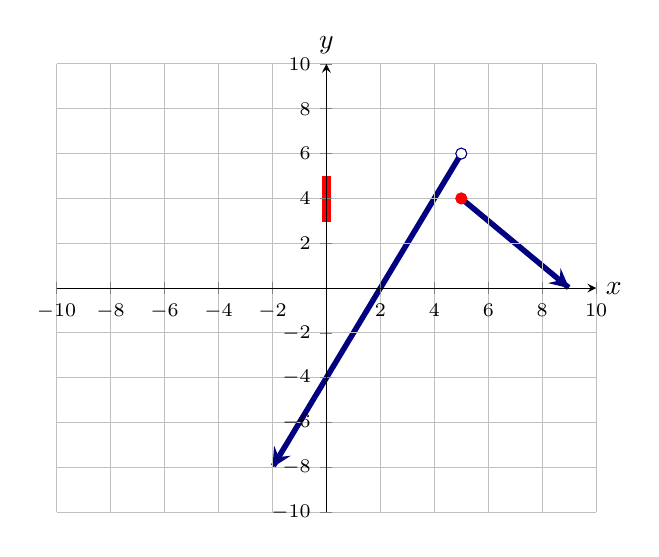
\begin{tikzpicture}
  \begin{axis}[
            domain=-10:10, ymax=10, xmax=10, ymin=-10, xmin=-10,
            axis lines =center, xlabel=$x$, ylabel=$y$, grid = major,
            ytick={-10,-8,-6,-4,-2,2,4,6,8,10},
            xtick={-10,-8,-6,-4,-2,2,4,6,8,10},
            ticklabel style={font=\scriptsize},
            every axis y label/.style={at=(current axis.above origin),anchor=south},
            every axis x label/.style={at=(current axis.right of origin),anchor=west},
            axis on top
          ]
          
          \addplot [line width=2, penColor, smooth,samples=200,domain=(-2:5),<-] {2*x-4};
          \addplot [line width=2, penColor, smooth,samples=200,domain=(5:9),->] {-x+9};

          \addplot[color=red,fill=red,only marks,mark=*] coordinates{(5,4)};
          \addplot[color=penColor,fill=white,only marks,mark=*] coordinates{(5,6)};

          \addplot [line width=3, red, smooth,samples=200,domain=(3:5)] ({0},{x});

  \end{axis}
\end{tikzpicture}
\end{image}





$\vartriangleright$ Can we select an interval CONTAINING $5$, small enough, so that all domain numbers inside this interval have their function values inside $(3,5)$?  The answer is yes.

Select $[5, 6)$. \\



$\vartriangleright$ Can we select an \textbf{\textcolor{red!70!black}{OPEN}} interval containing $5$, small enough, so that all domain numbers inside this interval have their function values inside $(3,5)$?  The answer is \textbf{no}.




Let $0.1 > \delta > 0$ be a number as small as you wish.

Consider the open interval $(5-\delta, 5+\delta)$ around $5$. It doesn't matter how small $\delta$ is.  The number $5 - \frac{\delta}{2}$ is always inside this open interval and the function value there is 

\[  f\left(5 - \frac{\delta}{2}\right)     = 2\left(5 - \frac{\delta}{2}\right)-4 = 6 - \delta     \]



\begin{image}
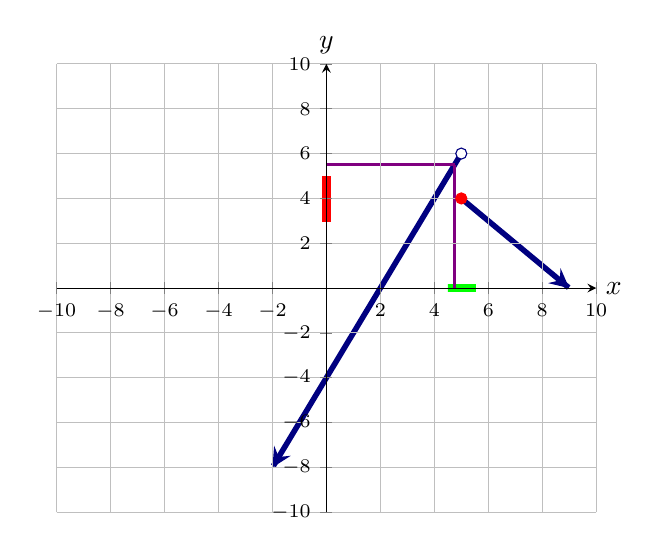
\begin{tikzpicture}
  \begin{axis}[
            domain=-10:10, ymax=10, xmax=10, ymin=-10, xmin=-10,
            axis lines =center, xlabel=$x$, ylabel=$y$, grid = major,
            ytick={-10,-8,-6,-4,-2,2,4,6,8,10},
            xtick={-10,-8,-6,-4,-2,2,4,6,8,10},
            ticklabel style={font=\scriptsize},
            every axis y label/.style={at=(current axis.above origin),anchor=south},
            every axis x label/.style={at=(current axis.right of origin),anchor=west},
            axis on top
          ]
          
          \addplot [line width=2, penColor, smooth,samples=200,domain=(-2:5),<-] {2*x-4};
          \addplot [line width=2, penColor, smooth,samples=200,domain=(5:9),->] {-x+9};


          \addplot[color=red,fill=red,only marks,mark=*] coordinates{(5,4)};
          \addplot[color=penColor,fill=white,only marks,mark=*] coordinates{(5,6)};

          \addplot [line width=3, red, smooth,samples=200,domain=(3:5)] ({0},{x});
          \addplot [line width=3, green, smooth,samples=200,domain=(4.5:5.5)] ({x},{0});

          \addplot [line width=1, violet, smooth,samples=200,domain=(0:5.5)] ({4.75},{x});
          \addplot [line width=1, violet, smooth,samples=200,domain=(0:4.75)] ({x},{5.5});

  \end{axis}
\end{tikzpicture}
\end{image}



Since $0.1 > \delta$, we know for sure that $6 - \delta > 5$.  \\
$6 - \delta$ is \textbf{\textcolor{red!70!black}{NEVER}} inside $(3, 5)$, for \textbf{\textcolor{red!70!black}{ANY}} $\delta$.\\



There is no \textbf{open} interval around $5$, such that all function values of all domain numbers inside this interval are always inside $(3,5)$. \\




We have produced an $\epsilon$, such that there is no open interval around $5$ where the function values of domain numbers inside this interval are always inside $(4-\epsilon , 4+\epsilon)$.


That is, algebraically, what is means to be a discontinuity.



\end{explanation}
\end{example}













\begin{warning} \textbf{\textcolor{red!70!black}{You are Assuming Something}}

Read the definition again. \\

It did not say that the $\epsilon$-interval would be totally inside the range. \\

It did not say that the $\delta$-interval would be totally inside the domain. \\

\end{warning}


The following two examples will illustrate this.
























\begin{example}


\[
\text{Let } \, K(t) = 
\begin{cases}
  2t-8 & \text{ on } (-2, 5) \\
  7   & \text{ at } 5 \\
  -t + 9  & \text{ on } (5, 9)
\end{cases}
\]



Graph of $y=K(t)$


\begin{image}
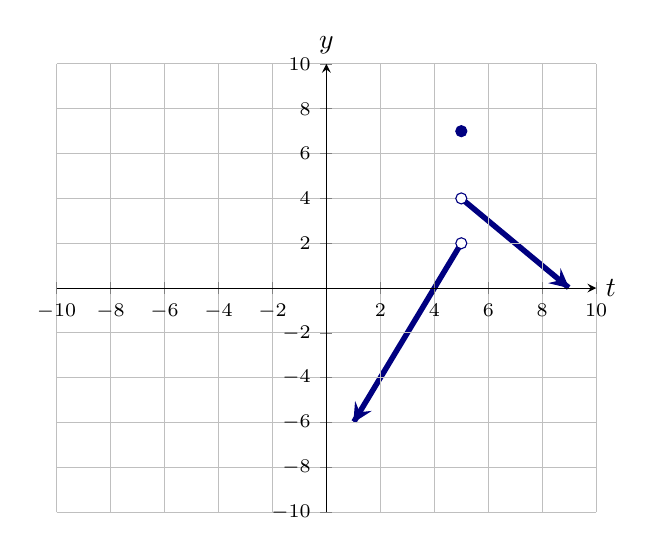
\begin{tikzpicture}
  \begin{axis}[
            domain=-10:10, ymax=10, xmax=10, ymin=-10, xmin=-10,
            axis lines =center, xlabel={$t$}, ylabel={$y$}, grid = major,
            ytick={-10,-8,-6,-4,-2,2,4,6,8,10},
            xtick={-10,-8,-6,-4,-2,2,4,6,8,10},
            ticklabel style={font=\scriptsize},
            every axis y label/.style={at=(current axis.above origin),anchor=south},
            every axis x label/.style={at=(current axis.right of origin),anchor=west},
            axis on top
          ]
          
          \addplot [line width=2, penColor, smooth,samples=200,domain=(1:5),<-] {2*x-8};
          \addplot [line width=2, penColor, smooth,samples=200,domain=(5:9),->] {-x+9};

          \addplot[color=penColor,fill=white,only marks,mark=*] coordinates{(5,4)};
          \addplot[color=penColor,fill=white,only marks,mark=*] coordinates{(5,2)};

          \addplot[color=penColor,fill=penColor,only marks,mark=*] coordinates{(5,7)};

  \end{axis}
\end{tikzpicture}
\end{image}


$5$ is a disconinuity of $K$. \\



\begin{explanation}


First, $5$ is in the domain and $f(5)=7$ is in the range.  Our plan is to pick an open interval around $7$ and show that no matter how close you get to $5$ in the domain, there is always a domain number whose function value is not inside our interval.


For our selection, pick a radius of $\epsilon = 1$ and consider the interval $(7-\epsilon , 7+\epsilon) = (7-1 , 7+1) = (6,8)$. \\


\begin{image}
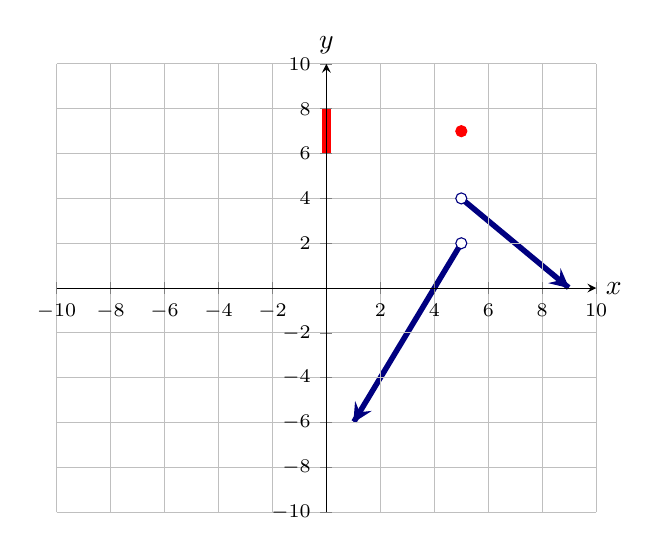
\begin{tikzpicture}
  \begin{axis}[
            domain=-10:10, ymax=10, xmax=10, ymin=-10, xmin=-10,
            axis lines =center, xlabel=$x$, ylabel=$y$, grid = major,
            ytick={-10,-8,-6,-4,-2,2,4,6,8,10},
            xtick={-10,-8,-6,-4,-2,2,4,6,8,10},
            ticklabel style={font=\scriptsize},
            every axis y label/.style={at=(current axis.above origin),anchor=south},
            every axis x label/.style={at=(current axis.right of origin),anchor=west},
            axis on top
          ]        

          \addplot [line width=2, penColor, smooth,samples=200,domain=(1:5),<-] {2*x-8};
          \addplot [line width=2, penColor, smooth,samples=200,domain=(5:9),->] {-x+9};

          \addplot[color=red,fill=red,only marks,mark=*] coordinates{(5,7)};
          \addplot[color=penColor,fill=white,only marks,mark=*] coordinates{(5,2)};
          \addplot[color=penColor,fill=white,only marks,mark=*] coordinates{(5,4)};

          \addplot [line width=3, red, smooth,samples=200,domain=(6:8)] ({0},{x});


  \end{axis}
\end{tikzpicture}
\end{image}



$\vartriangleright$ Can we select an \textbf{\textcolor{red!70!black}{OPEN}} interval containing $5$, small enough, so that all domain numbers inside this interval have their function values inside $(-4,-3)$?  The answer is \textbf{no}.




Let $0.1 > \delta > 0$ be a number as small as you wish.

Consider the open interval $(5-\delta, 5+\delta)$ around $5$. It doesn't matter how small $\delta$ is.  The number $5 - \frac{\delta}{2}$ is always inside this open interval and the function value there is 

\[  f\left(5 - \frac{\delta}{2}\right)     = 2\left(5 - \frac{\delta}{2}\right)-8 = 2 - \delta     \]



\begin{image}
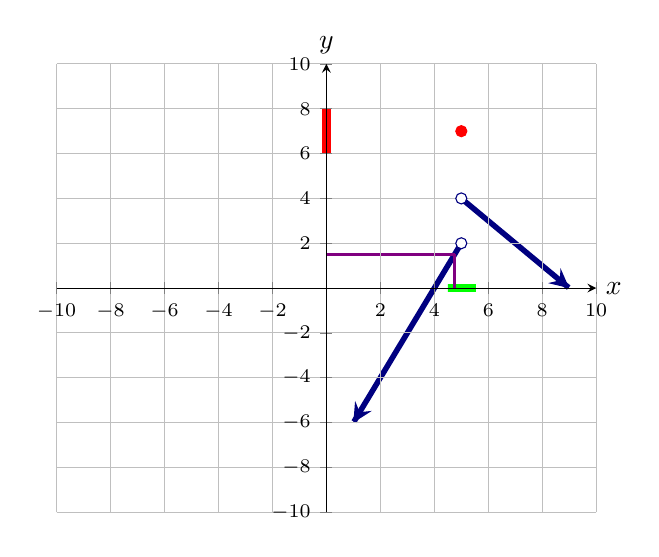
\begin{tikzpicture}
  \begin{axis}[
            domain=-10:10, ymax=10, xmax=10, ymin=-10, xmin=-10,
            axis lines =center, xlabel=$x$, ylabel=$y$, grid = major,
            ytick={-10,-8,-6,-4,-2,2,4,6,8,10},
            xtick={-10,-8,-6,-4,-2,2,4,6,8,10},
            ticklabel style={font=\scriptsize},
            every axis y label/.style={at=(current axis.above origin),anchor=south},
            every axis x label/.style={at=(current axis.right of origin),anchor=west},
            axis on top
          ]
                   
          \addplot [line width=2, penColor, smooth,samples=200,domain=(1:5),<-] {2*x-8};
          \addplot [line width=2, penColor, smooth,samples=200,domain=(5:9),->] {-x+9};

          \addplot[color=red,fill=red,only marks,mark=*] coordinates{(5,7)};
          \addplot[color=penColor,fill=white,only marks,mark=*] coordinates{(5,2)};
          \addplot[color=penColor,fill=white,only marks,mark=*] coordinates{(5,4)};

          \addplot [line width=3, red, smooth,samples=200,domain=(6:8)] ({0},{x});

          \addplot [line width=3, green, smooth,samples=200,domain=(4.5:5.5)] ({x},{0});

          \addplot [line width=1, violet, smooth,samples=200,domain=(0:1.5)] ({4.75},{x});
          \addplot [line width=1, violet, smooth,samples=200,domain=(0:4.75)] ({x},{1.5});

  \end{axis}
\end{tikzpicture}
\end{image}



Since $0.1 > \delta$, we know for sure that $2 - \delta < 2$.  \\
$2 - \delta$ is \textbf{\textcolor{red!70!black}{NEVER}} inside $(6, 8)$, for \textbf{\textcolor{red!70!black}{ANY}} $\delta$.\\



There is no open interval around $5$, such that all function values of all domain numbers inside this interval are always inside $(6,8)$. \\




We have produced an $\epsilon$, such that there is no open interval around $5$ where the function values of domain numbers inside this interval are always inside $(7-\epsilon , 7+\epsilon)$.


That is, algebraically, what is means to be a discontinuity.



\end{explanation}
\end{example}


In this example, the $\epsilon$-interval, $(7-\epsilon, 7+\epsilon) = (6,8)$, was not inside the range of $K$.  In fact, this interval contained only one function value and that was $7$.




























\begin{example}


\[
\text{Let } \, B(r) = 
\begin{cases}
  7   & \text{ at } 5 \\
  -t + 9  & \text{ on } (5, 9)
\end{cases}
\]



Graph of $y=B(t)$


\begin{image}
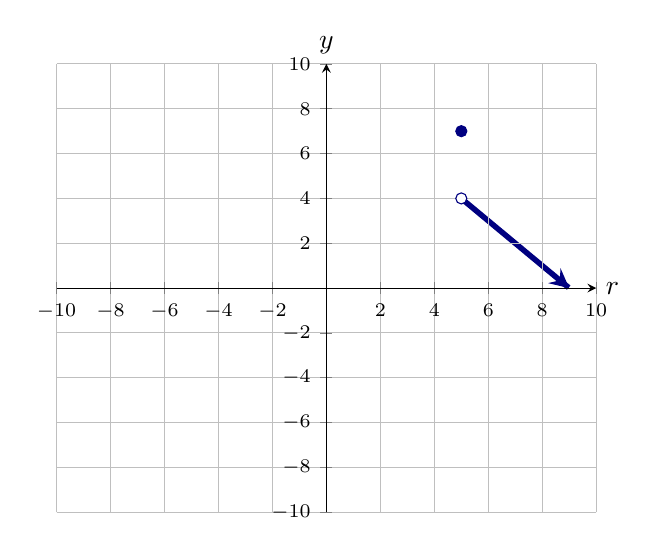
\begin{tikzpicture}
  \begin{axis}[
            domain=-10:10, ymax=10, xmax=10, ymin=-10, xmin=-10,
            axis lines =center, xlabel={$r$}, ylabel={$y$}, grid = major,
            ytick={-10,-8,-6,-4,-2,2,4,6,8,10},
            xtick={-10,-8,-6,-4,-2,2,4,6,8,10},
            ticklabel style={font=\scriptsize},
            every axis y label/.style={at=(current axis.above origin),anchor=south},
            every axis x label/.style={at=(current axis.right of origin),anchor=west},
            axis on top
          ]
          
          \addplot [line width=2, penColor, smooth,samples=200,domain=(5:9),->] {-x+9};

          \addplot[color=penColor,fill=white,only marks,mark=*] coordinates{(5,4)};

          \addplot[color=penColor,fill=penColor,only marks,mark=*] coordinates{(5,7)};

  \end{axis}
\end{tikzpicture}
\end{image}


$5$ is a disconinuity of $B$. \\



\begin{explanation}


First, $5$ is in the domain and $f(5)=7$ is in the range.  Our plan is to pick an open interval around $7$ and show that no matter how close you get to $5$ in the domain, there is always a domain number whose function value is not inside our interval.


For our selection, pick a radius of $\epsilon = 1$ and consider the interval $(7-\epsilon , 7+\epsilon) = (7-1 , 7+1) = (6,8)$. \\


\begin{image}
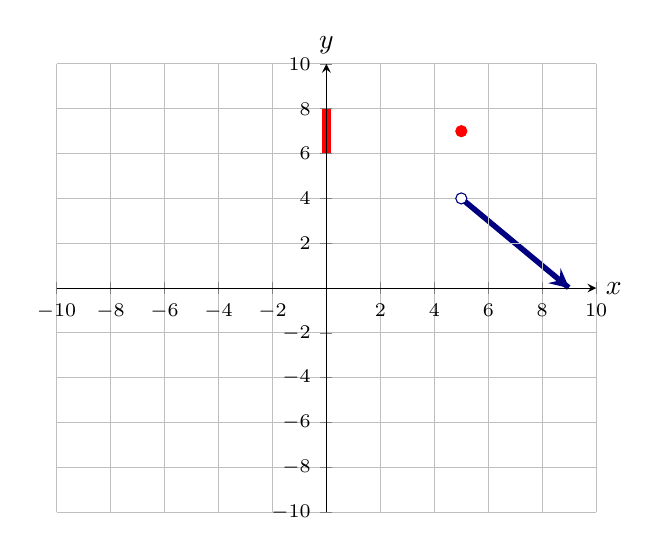
\begin{tikzpicture}
  \begin{axis}[
            domain=-10:10, ymax=10, xmax=10, ymin=-10, xmin=-10,
            axis lines =center, xlabel=$x$, ylabel=$y$, grid = major,
            ytick={-10,-8,-6,-4,-2,2,4,6,8,10},
            xtick={-10,-8,-6,-4,-2,2,4,6,8,10},
            ticklabel style={font=\scriptsize},
            every axis y label/.style={at=(current axis.above origin),anchor=south},
            every axis x label/.style={at=(current axis.right of origin),anchor=west},
            axis on top
          ]        

          \addplot [line width=2, penColor, smooth,samples=200,domain=(5:9),->] {-x+9};

          \addplot[color=red,fill=red,only marks,mark=*] coordinates{(5,7)};

          \addplot[color=penColor,fill=white,only marks,mark=*] coordinates{(5,4)};

          \addplot [line width=3, red, smooth,samples=200,domain=(6:8)] ({0},{x});


  \end{axis}
\end{tikzpicture}
\end{image}



$\vartriangleright$ Can we select an \textbf{\textcolor{red!70!black}{OPEN}} interval containing $5$, small enough, so that all domain numbers inside this interval have their function values inside $(6,8)$?  The answer is \textbf{no}.




Let $0.1 > \delta > 0$ be a number as small as you wish.

Consider the open interval $(5-\delta, 5+\delta)$ around $5$. It doesn't matter how small $\delta$ is.  The number $5 + \frac{\delta}{2}$ is always inside this open interval and the function value there is 

\[  f\left(5 + \frac{\delta}{2}\right)     = -\left(5 - \frac{\delta}{2}\right)+9 = 4 - \delta     \]



\begin{image}
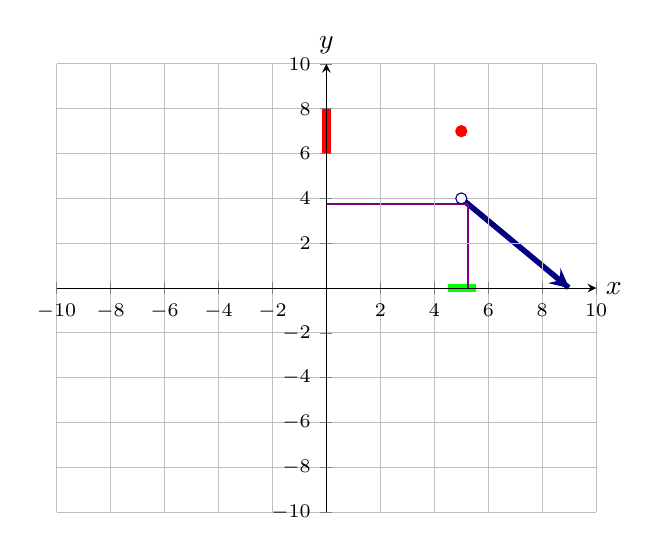
\begin{tikzpicture}
  \begin{axis}[
            domain=-10:10, ymax=10, xmax=10, ymin=-10, xmin=-10,
            axis lines =center, xlabel=$x$, ylabel=$y$, grid = major,
            ytick={-10,-8,-6,-4,-2,2,4,6,8,10},
            xtick={-10,-8,-6,-4,-2,2,4,6,8,10},
            ticklabel style={font=\scriptsize},
            every axis y label/.style={at=(current axis.above origin),anchor=south},
            every axis x label/.style={at=(current axis.right of origin),anchor=west},
            axis on top
          ]

          \addplot [line width=2, penColor, smooth,samples=200,domain=(5:9),->] {-x+9};

          \addplot[color=red,fill=red,only marks,mark=*] coordinates{(5,7)};
          \addplot[color=penColor,fill=white,only marks,mark=*] coordinates{(5,4)};

          \addplot [line width=3, red, smooth,samples=200,domain=(6:8)] ({0},{x});

          \addplot [line width=3, green, smooth,samples=200,domain=(4.5:5.5)] ({x},{0});

          \addplot [line width=1, violet, smooth,samples=200,domain=(0:3.75)] ({5.25},{x});
          \addplot [line width=1, violet, smooth,samples=200,domain=(0:5.25)] ({x},{3.75});

  \end{axis}
\end{tikzpicture}
\end{image}



Since $0.1 > \delta$, we know for sure that $4 - \delta < 4$.  \\
$4 - \delta$ is \textbf{\textcolor{red!70!black}{NEVER}} inside $(6, 8)$, for \textbf{\textcolor{red!70!black}{ANY}} $\delta$.\\



There is no open interval around $5$, such that all function values of all domain numbers inside this interval are always inside $(6,8)$. \\




We have produced an $\epsilon$, such that there is no open interval around $5$ where the function values of domain numbers inside this interval are always inside $(7-\epsilon , 7+\epsilon)$.


That is, algebraically, what is means to be a discontinuity.



\end{explanation}
\end{example}




























How about an example where the graph is not so easy to draw?













\begin{example}  Discontinuity


\[
\text{Let } \, T(k) = 
\begin{cases}
  0 & \text{ on } \mathbb{R} - \left\{ \frac{1}{n} \, | \, n \in \mathbb{N}     \right\} \\
  1  & \text{ on } \left\{ \frac{1}{n} \, | \, n \in \mathbb{N}     \right\}
\end{cases}
\]



Claim: $0$ is a discontinuity of $f$. \\



\begin{explanation}

$T(k)$ is $0$ everywhere except the reciprocals of the natural numbers.

The natural numbers are $\{ 1, 2, 3, 4, \cdots \}$.

The reciprocals of the natural numbers are $\left\{ 1, \frac{1}{2}, \frac{1}{3}, \frac{1}{4}, \cdots \right\}$.

On the reciprocals, $f\left(\frac{1}{n}\right) = 1$ \\



First, $0$ is in the domain and $f(0) = 0$.

Second, for any small $0.1 > \epsilon > 0$ choosen, the interval $(-\epsilon, \epsilon)$ is an open interval around $f(0) = 0$. \\



Now, consider any $\delta > 0$ and the interval $(-\delta, \delta)$. No mater how small $\delta$ is, there is an $n_0 \in \mathbb{N}$, such that $0 < \frac{1}{n_0} < \delta$ and $f\left(\frac{1}{n_0}\right) = 1$, which is outside $(-\epsilon, \epsilon)$. \\




For \textbf{\textcolor{red!50!blue!90!black}{ANY}} choosen $\epsilon$-interval around $f(0)= 0$, there is no corresponding $\delta$ such that \textbf{\textcolor{red!50!blue!90!black}{ALL}} of the function values from  $(-\delta, \delta)$ land inside $(-\epsilon, \epsilon)$.


$0$ is a discontinuity of $f$.

\end{explanation}

\end{example}






In the example above, $T(k)$ didn't have a big space surrounding the function value.  Instead it just had an infinite number of single individual values jump away from the target value.


The example demonstrates that functions do just about any and every weird thing you can think of.













\section*{Naming Discontinuities}



We want language for discontinuities.  We want words we can say that give people an idea of our thoughts. We want algebraic language to be exact about our thoughts.


We'll start with \textbf{jump}, \textbf{removeable}, and \textbf{asymptotic}.



\begin{example} \textbf{\textcolor{blue!55!black}{Jump Discontinuity}}



A jump discontinuity occurs when the function is continuous to the left and right side of the discontinuity, but the two sides do not match up.



The function must be defined for a discontinuity.  The corresponding point could be an endpoint for either side or neither.



\begin{image}
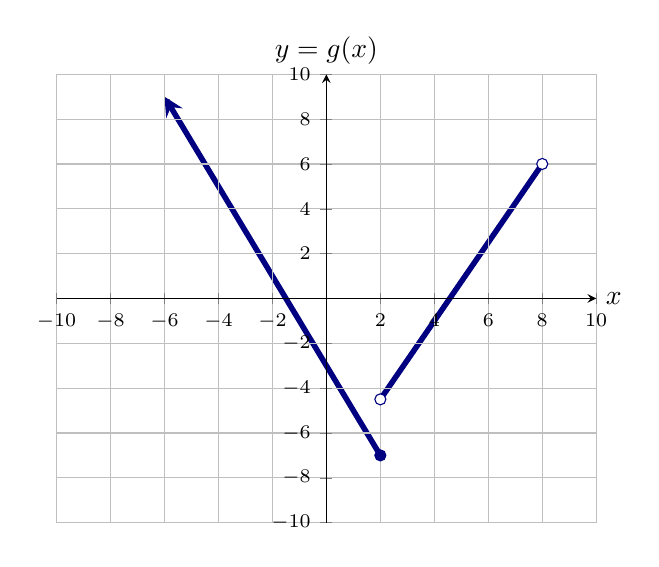
\begin{tikzpicture}
  \begin{axis}[
            domain=-10:10, ymax=10, xmax=10, ymin=-10, xmin=-10,
            axis lines =center, xlabel=$x$, ylabel={$y=g(x)$}, grid = major,
            ytick={-10,-8,-6,-4,-2,2,4,6,8,10},
          	xtick={-10,-8,-6,-4,-2,2,4,6,8,10},
          	yticklabels={$-10$,$-8$,$-6$,$-4$,$-2$,$2$,$4$,$6$,$8$,$10$}, 
          	xticklabels={$-10$,$-8$,$-6$,$-4$,$-2$,$2$,$4$,$6$,$8$,$10$},
            ticklabel style={font=\scriptsize},
            every axis y label/.style={at=(current axis.above origin),anchor=south},
            every axis x label/.style={at=(current axis.right of origin),anchor=west},
            axis on top
          ]
          
      		\addplot [line width=2, penColor, smooth,samples=100,domain=(-6:2),<-] {-2*x-3};
          \addplot [line width=2, penColor, smooth,samples=100,domain=(2:8)] {1.75*x-8};

      		\addplot[color=penColor,fill=penColor,only marks,mark=*] coordinates{(2,-7)};

      		\addplot[color=penColor,fill=white,only marks,mark=*] coordinates{(2,-4.5)};
      		\addplot[color=penColor,fill=white,only marks,mark=*] coordinates{(8,6)};


           

  \end{axis}
\end{tikzpicture}
\end{image}





\begin{image}
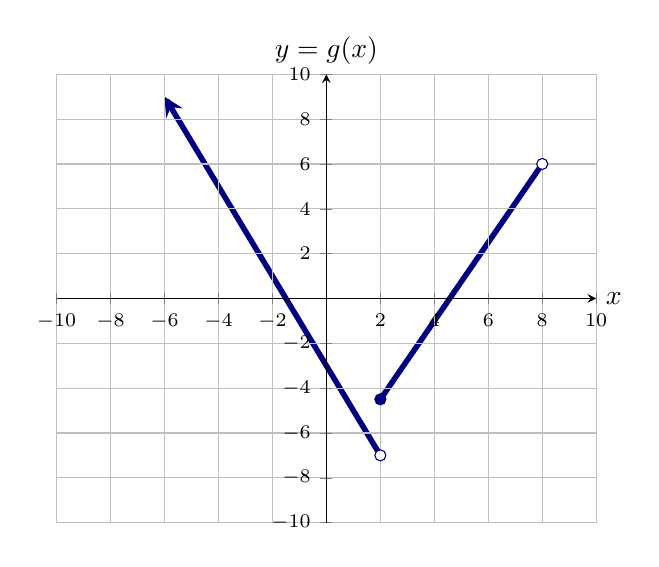
\begin{tikzpicture}
  \begin{axis}[
            domain=-10:10, ymax=10, xmax=10, ymin=-10, xmin=-10,
            axis lines =center, xlabel=$x$, ylabel={$y=g(x)$}, grid = major,
            ytick={-10,-8,-6,-4,-2,2,4,6,8,10},
          	xtick={-10,-8,-6,-4,-2,2,4,6,8,10},
          	yticklabels={$-10$,$-8$,$-6$,$-4$,$-2$,$2$,$4$,$6$,$8$,$10$}, 
          	xticklabels={$-10$,$-8$,$-6$,$-4$,$-2$,$2$,$4$,$6$,$8$,$10$},
            ticklabel style={font=\scriptsize},
            every axis y label/.style={at=(current axis.above origin),anchor=south},
            every axis x label/.style={at=(current axis.right of origin),anchor=west},
            axis on top
          ]
          
      		\addplot [line width=2, penColor, smooth,samples=100,domain=(-6:2),<-] {-2*x-3};
          \addplot [line width=2, penColor, smooth,samples=100,domain=(2:8)] {1.75*x-8};

      		\addplot[color=penColor,fill=white,only marks,mark=*] coordinates{(2,-7)};

      		\addplot[color=penColor,fill=penColor,only marks,mark=*] coordinates{(2,-4.5)};
      		\addplot[color=penColor,fill=white,only marks,mark=*] coordinates{(8,6)};


           

  \end{axis}
\end{tikzpicture}
\end{image}



Or, the point could be off on its own, isolated.



\begin{image}
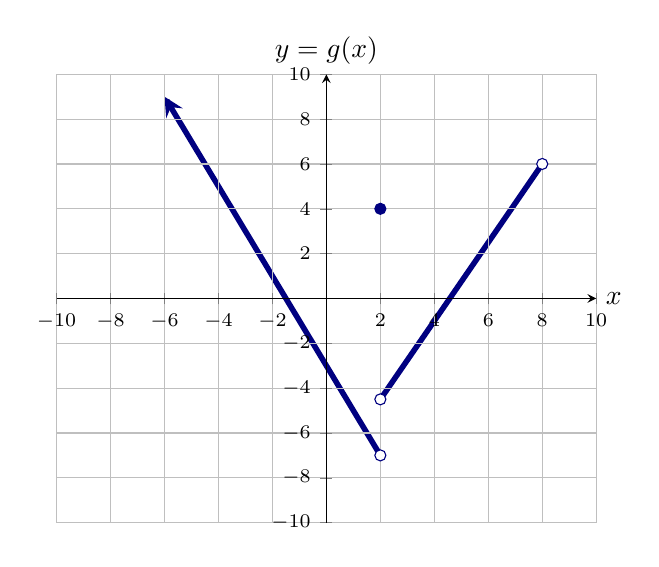
\begin{tikzpicture}
  \begin{axis}[
            domain=-10:10, ymax=10, xmax=10, ymin=-10, xmin=-10,
            axis lines =center, xlabel=$x$, ylabel={$y=g(x)$}, grid = major,
            ytick={-10,-8,-6,-4,-2,2,4,6,8,10},
          	xtick={-10,-8,-6,-4,-2,2,4,6,8,10},
          	yticklabels={$-10$,$-8$,$-6$,$-4$,$-2$,$2$,$4$,$6$,$8$,$10$}, 
          	xticklabels={$-10$,$-8$,$-6$,$-4$,$-2$,$2$,$4$,$6$,$8$,$10$},
            ticklabel style={font=\scriptsize},
            every axis y label/.style={at=(current axis.above origin),anchor=south},
            every axis x label/.style={at=(current axis.right of origin),anchor=west},
            axis on top
          ]
          
      		\addplot [line width=2, penColor, smooth,samples=100,domain=(-6:2),<-] {-2*x-3};
          \addplot [line width=2, penColor, smooth,samples=100,domain=(2:8)] {1.75*x-8};


      		\addplot[color=penColor,fill=penColor,only marks,mark=*] coordinates{(2,4)};

      		\addplot[color=penColor,fill=white,only marks,mark=*] coordinates{(2,-4.5)};
      		\addplot[color=penColor,fill=white,only marks,mark=*] coordinates{(8,6)};
      		\addplot[color=penColor,fill=white,only marks,mark=*] coordinates{(2,-7)};


           

  \end{axis}
\end{tikzpicture}
\end{image}




\end{example} 





























\begin{example} \textbf{\textcolor{blue!55!black}{Removeable Discontinuity}} 



A removeable discontinuity occurs when the function is continuous to the left and right side of the discontinuity, and the two sides do match up.  However, the point at the discontinuity is moved, leaving a hole.






\begin{image}
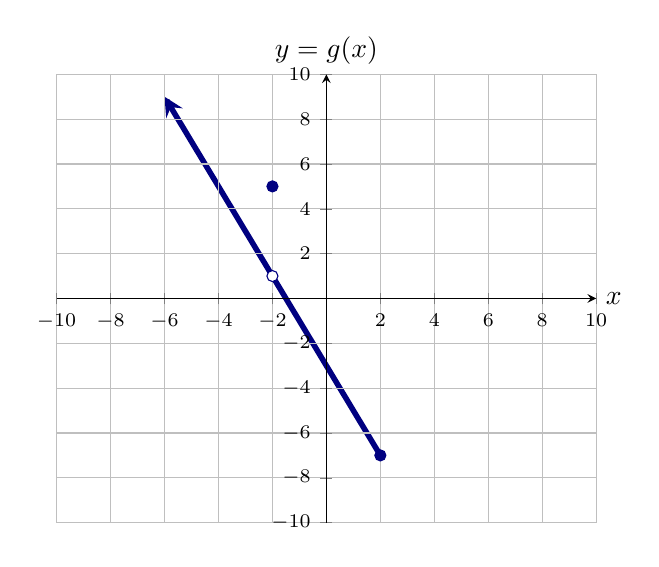
\begin{tikzpicture}
  \begin{axis}[
            domain=-10:10, ymax=10, xmax=10, ymin=-10, xmin=-10,
            axis lines =center, xlabel=$x$, ylabel={$y=g(x)$}, grid = major,
            ytick={-10,-8,-6,-4,-2,2,4,6,8,10},
          	xtick={-10,-8,-6,-4,-2,2,4,6,8,10},
          	yticklabels={$-10$,$-8$,$-6$,$-4$,$-2$,$2$,$4$,$6$,$8$,$10$}, 
          	xticklabels={$-10$,$-8$,$-6$,$-4$,$-2$,$2$,$4$,$6$,$8$,$10$},
            ticklabel style={font=\scriptsize},
            every axis y label/.style={at=(current axis.above origin),anchor=south},
            every axis x label/.style={at=(current axis.right of origin),anchor=west},
            axis on top
          ]
          
      		\addplot [line width=2, penColor, smooth,samples=100,domain=(-6:2),<-] {-2*x-3};

      		\addplot[color=penColor,fill=penColor,only marks,mark=*] coordinates{(2,-7)};

      		\addplot[color=penColor,fill=white,only marks,mark=*] coordinates{(-2,1)};
      		\addplot[color=penColor,fill=penColor,only marks,mark=*] coordinates{(-2,5)};


           

  \end{axis}
\end{tikzpicture}
\end{image}




\end{example}

This type of discontinuity can be ``removed'' simply by redefining the function value at that one number and moving the point back onto the graph to plug the hole.




\begin{image}
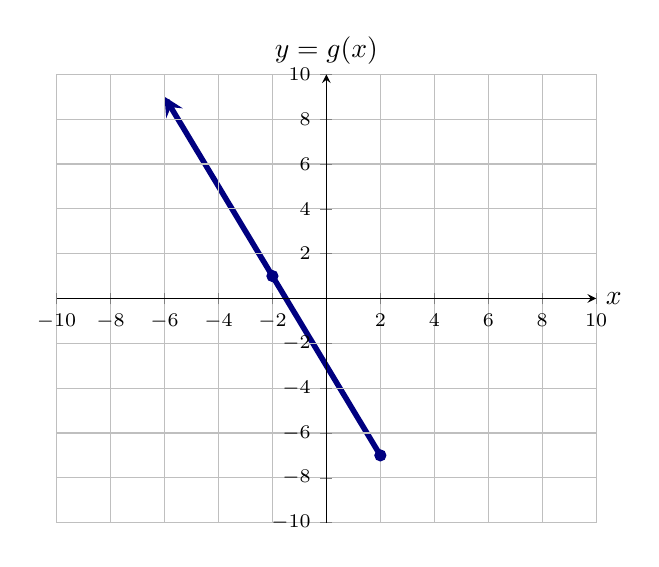
\begin{tikzpicture}
  \begin{axis}[
            domain=-10:10, ymax=10, xmax=10, ymin=-10, xmin=-10,
            axis lines =center, xlabel=$x$, ylabel={$y=g(x)$}, grid = major,
            ytick={-10,-8,-6,-4,-2,2,4,6,8,10},
          	xtick={-10,-8,-6,-4,-2,2,4,6,8,10},
          	yticklabels={$-10$,$-8$,$-6$,$-4$,$-2$,$2$,$4$,$6$,$8$,$10$}, 
          	xticklabels={$-10$,$-8$,$-6$,$-4$,$-2$,$2$,$4$,$6$,$8$,$10$},
            ticklabel style={font=\scriptsize},
            every axis y label/.style={at=(current axis.above origin),anchor=south},
            every axis x label/.style={at=(current axis.right of origin),anchor=west},
            axis on top
          ]
          
      		\addplot [line width=2, penColor, smooth,samples=100,domain=(-6:2),<-] {-2*x-3};

      		\addplot[color=penColor,fill=penColor,only marks,mark=*] coordinates{(2,-7)};

      		\addplot[color=penColor,fill=penColor,only marks,mark=*] coordinates{(-2,1)};

  \end{axis}
\end{tikzpicture}
\end{image}


































\begin{example} \textbf{\textcolor{blue!55!black}{Asymptotic Discontinuity}} 


The third type of discontinuity is when the values of function become unbounded near a domain number.  Graphically, these are represented with asymptotes.  There are several possible configurations.



Discontinuities where both sides become unbounded.



\begin{image}
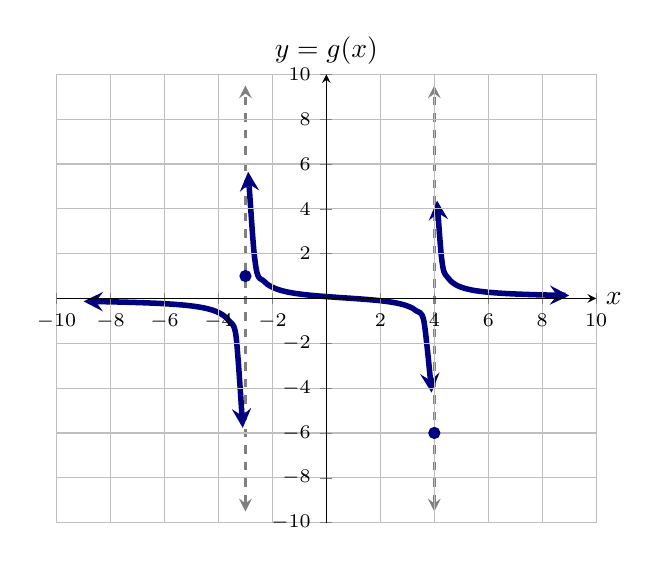
\begin{tikzpicture}
  \begin{axis}[
            domain=-10:10, ymax=10, xmax=10, ymin=-10, xmin=-10,
            axis lines =center, xlabel=$x$, ylabel={$y=g(x)$}, grid = major,
            ytick={-10,-8,-6,-4,-2,2,4,6,8,10},
          	xtick={-10,-8,-6,-4,-2,2,4,6,8,10},
          	yticklabels={$-10$,$-8$,$-6$,$-4$,$-2$,$2$,$4$,$6$,$8$,$10$}, 
          	xticklabels={$-10$,$-8$,$-6$,$-4$,$-2$,$2$,$4$,$6$,$8$,$10$},
            ticklabel style={font=\scriptsize},
            every axis y label/.style={at=(current axis.above origin),anchor=south},
            every axis x label/.style={at=(current axis.right of origin),anchor=west},
            axis on top
          ]

          \addplot [line width=1, gray, dashed, domain=(-9.5:9.5),<->] ({-3},{x});
          \addplot [line width=1, gray, dashed, domain=(-9.5:9.5),<->] ({4},{x});

          \addplot [line width=2, penColor, smooth, domain=(-9:-3.1),<->] {(x-1)/((x+3)*(x-4))};
          \addplot [line width=2, penColor, smooth, domain=(-2.9:3.9),<->] {(x-1)/((x+3)*(x-4))};
          \addplot [line width=2, penColor, smooth, domain=(4.1:9),<->] {(x-1)/((x+3)*(x-4))};


      		\addplot[color=penColor,fill=penColor,only marks,mark=*] coordinates{(-3,1)};
      		\addplot[color=penColor,fill=penColor,only marks,mark=*] coordinates{(4,-6)};


  \end{axis}
\end{tikzpicture}
\end{image}






Discontinuities where only one side becomes unbounded.



\begin{image}
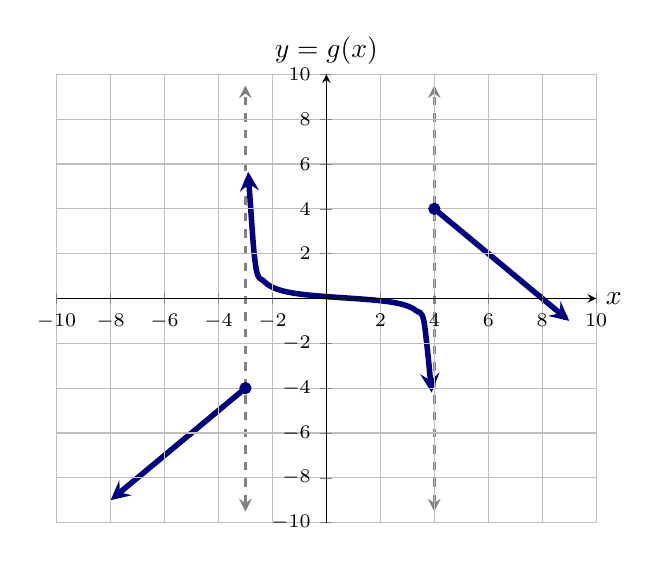
\begin{tikzpicture}
  \begin{axis}[
            domain=-10:10, ymax=10, xmax=10, ymin=-10, xmin=-10,
            axis lines =center, xlabel=$x$, ylabel={$y=g(x)$}, grid = major,
            ytick={-10,-8,-6,-4,-2,2,4,6,8,10},
          	xtick={-10,-8,-6,-4,-2,2,4,6,8,10},
          	yticklabels={$-10$,$-8$,$-6$,$-4$,$-2$,$2$,$4$,$6$,$8$,$10$}, 
          	xticklabels={$-10$,$-8$,$-6$,$-4$,$-2$,$2$,$4$,$6$,$8$,$10$},
            ticklabel style={font=\scriptsize},
            every axis y label/.style={at=(current axis.above origin),anchor=south},
            every axis x label/.style={at=(current axis.right of origin),anchor=west},
            axis on top
          ]

          \addplot [line width=1, gray, dashed, domain=(-9.5:9.5),<->] ({-3},{x});
          \addplot [line width=1, gray, dashed, domain=(-9.5:9.5),<->] ({4},{x});

          \addplot [line width=2, penColor, smooth, domain=(-8:-3),<-] {x-1};
          \addplot [line width=2, penColor, smooth, domain=(-2.9:3.9),<->] {(x-1)/((x+3)*(x-4))};
          \addplot [line width=2, penColor, smooth, domain=(4.1:9),->] {-x+8};

      		\addplot[color=penColor,fill=penColor,only marks,mark=*] coordinates{(-3,-4)};
      		\addplot[color=penColor,fill=penColor,only marks,mark=*] coordinates{(4,4)};


  \end{axis}
\end{tikzpicture}
\end{image}





\end{example}







Those are the three main types of discontinuities we will encounter.  Usually, we use piecewise defined functions to create discontiuities.











\begin{center}
\textbf{\textcolor{green!50!black}{ooooo-=-=-=-ooOoo-=-=-=-ooooo}} \\

more examples can be found by following this link\\ \link[More Examples of Continuity]{https://ximera.osu.edu/csccmathematics/precalculus1/precalculus1/continuity/examples/exampleList}

\end{center}






\end{document}
